\documentclass[10pt,letterpaper]{article}
\usepackage[margin=0.67in]{geometry}
\usepackage[T1]{fontenc}
\usepackage{lmodern,microtype,amsmath,amssymb,booktabs,array,graphicx,enumitem}
\usepackage{xcolor,hyperref,fancyhdr,caption}
\definecolor{ink}{HTML}{24517E}
\hypersetup{colorlinks=true,urlcolor=ink,linkcolor=ink,pdftitle={Optimizing neural wavefunctions for strongly correlated quantum systems},pdfauthor={PassengerAn}}
\pagestyle{fancy}\fancyhf{}
\fancyhead[L]{\small Applied Machine Learning: project proposal}
\fancyhead[R]{\small PassengerAn \textbar\ 23 October 2026}
\fancyfoot[C]{\thepage}
\setlength{\headheight}{13pt}
\setlength{\parindent}{0pt}\setlength{\parskip}{4pt}
\setlength{\emergencystretch}{2em}
\setlength{\abovedisplayskip}{5pt}\setlength{\belowdisplayskip}{5pt}
\setlist{leftmargin=15pt,itemsep=3pt,topsep=3pt}
\captionsetup{font=small,labelfont=bf}
\newcommand{\topic}[1]{\vspace{4pt}\textbf{\color{ink}#1}\par}
\newcommand{\avg}[1]{\langle #1\rangle}
\newcommand{\R}{\mathbb R}
% Generated from verified benchmark records; do not edit numerical rows by hand.
\newcommand{\FQHEDatabaseRows}{4 & $18\times10$ & 0.680604 \\
5 & $73\times13$ & 0.609317 \\
6 & $338\times16$ & 0.585780 \\
7 & $1,656\times19$ & 0.548749 \\
8 & $8,512\times22$ & 0.531577 \\}
\newcommand{\IsingDatabaseRows}{4 & $16\times4$ & -5.226252 & 0.397825 \\
6 & $64\times6$ & -7.727407 & 0.263305 \\
8 & $256\times8$ & -10.251662 & 0.196983 \\
10 & $1,024\times10$ & -12.784906 & 0.157403 \\}
\newcommand{\ArchitectureRows}{MLP & 23,042 & 0.499735 & 0.354091 \\
Dense correction & 24,606 & 0.491581 & 0.362938 \\
Attention correction & 24,596 & 0.504275 & 0.346992 \\}
\newcommand{\IsingEDZero}{-7.727406610313}
\newcommand{\FQHEGap}{0.531576795}
\newcommand{\IsingFidelity}{0.999998569}
\newcommand{\FQHEFidelity}{0.365698814}
\newcommand{\FQHEEnergy}{0.490844981}
\newcommand{\IsingConfigRows}{1,488}
\newcommand{\FQHEConfigRows}{10,597}
\newcommand{\TotalConfigRows}{12,085}
\newcommand{\IsingLogShape}{52\times9}
\newcommand{\FQHELogShape}{20\times7}
\newcommand{\FQHEEndpointShape}{6\times26}

\begin{document}
\begin{center}
{\Large\bfseries Optimizing neural wavefunctions for\\strongly correlated quantum systems}\par
\vspace{3pt}
\ifdefined\OutlineOnly
{\small Project outline; supplementary workflow and benchmarks are available in the repository}
\else
{\small Two-page proposal; workflow and benchmark examples follow in appendices}
\fi
\end{center}

\textbf{Research question.} Which optimization strategies learn neural wavefunctions efficiently as we progress from a simple quantum spin model to strongly correlated fermionic systems? We will compare \textbf{SPRING, SR/MinSR, K-FAC and Adam}, with SGD as a simple control, using \textbf{Ising as the entry-level benchmark and Hubbard or FQHE as an advanced extension}. \emph{Variational Monte Carlo (VMC) is the common training framework}; the optimizers are alternatives inside it. Our hypothesis is that SPRING's retained geometric direction helps noisy, small-batch optimization, with benefits that depend on correlations, sign/phase structure and solver cost. The contribution is a controlled benchmark of accuracy, efficiency and transfer across problem difficulty.

\topic{1. Physics supplies the wavefunction family; ML learns its coefficients}
The prediction task is to learn a structured wavefunction and its physical observables from a known Hamiltonian, without supervised ground-state labels. Domain knowledge determines the Hilbert space, basis, symmetries and allowed functional form; it does not supply the exact solution. In a physical basis $\mathcal B$, a general representation is
\begin{equation}
 |\Psi_\theta\rangle=\sum_{x\in\mathcal B}e^{a_\theta(x)+ib_\theta(x)}|x\rangle_{\rm phys}.
\end{equation}
The NN learns amplitude and, where needed, sign/phase information. Choose an appropriate ansatz for each system, then keep it fixed across optimizer comparisons [1,2].

\textbf{Entry level: Ising model.} Begin with the periodic transverse-field chain
$H_{\mathrm I}=-J\sum_i Z_iZ_{i+1}-h\sum_iX_i$, using Pauli eigenvalues $s_i=\pm1$.
The input is a spin configuration; the output is its real log amplitude. The existing RBM,
$\log\psi_\theta(s)=c+\sum_a\log\cosh(\sum_i s_iW_{ia})$, enforces positivity and even global spin-flip parity, appropriate for $h>0$. Small chains ($N=6,10$) provide inexpensive checks of gradients, curvature and convergence before advanced fermionic work.

\textbf{Advanced option A: Hubbard model.} The repulsive single-band model [8] is
\begin{equation}
 H_{\mathrm H}=-t\sum_{\langle i,j\rangle,\sigma}
 (c^\dagger_{i\sigma}c_{j\sigma}+\mathrm{h.c.})+U\sum_i n_{i\uparrow}n_{i\downarrow},\qquad U>0.
\end{equation}
Start with an ED-accessible $2\times2$ cluster at half filling and specified open boundaries, fixing $N_\uparrow=N_\downarrow=2$. Inputs are spin-resolved occupations. A canonically ordered fermionic basis enforces antisymmetry; the NN learns signed or complex coefficients. Larger clusters and stronger $U/t$ are follow-up tests after validation. Hubbard ED and neural calculations are proposed work.

\textbf{Advanced option B: FQHE.} An alternative is the existing spin-polarized spherical LLL benchmark, $H/V_1=\sum_{i<j}P_{R=1}(i,j)$, at $N_\phi=3(N-1)$ and fixed $L_z=0$. Occupation inputs and antisymmetric Slater states define the representation; the NN learns complex coefficients. Existing small-system ED and NN examples support this option. We will select \emph{one} advanced model after the Ising study; broader FQHE Hamiltonians [7] are later extensions.

\topic{2. Shared energy loss, sampled gradients and optimizer alternatives}
For any chosen system and configuration $x$, the common objective and Born probability are
\begin{equation}
 \mathcal L(\theta)=\frac{\langle\Psi_\theta|H|\Psi_\theta\rangle}
 {\langle\Psi_\theta|\Psi_\theta\rangle}
 =\mathbb E_{p_\theta}[\operatorname{Re}E_{\rm loc}(x)],\quad
 p_\theta(x)=\frac{|\psi_\theta(x)|^2}{\sum_{x'}|\psi_\theta(x')|^2},\quad
 E_{\rm loc}(x)=\sum_{x'}H_{xx'}\frac{\psi_\theta(x')}{\psi_\theta(x)} .
\end{equation}
For real parameters and $O_a=\partial_{\theta_a}\log\psi_\theta$, estimate
\begin{equation}
 g_a=2\operatorname{Re}\langle\delta O_a^*\delta E_{\rm loc}\rangle,
 \qquad S_{ab}=\operatorname{Re}\langle\delta O_a^*\delta O_b\rangle,
 \qquad \delta O=O-\langle O\rangle .
\end{equation}
SGD updates $\theta\leftarrow\theta-\eta g$; Adam adds adaptive first/second moments [6]. SR solves a damped geometric system, and MinSR uses its sample-space form [3]. SPRING reuses a previous raw direction across sampled solves [4]. K-FAC approximates layer curvature with Kronecker factors [5]. Real-state adapters are validated first; complex states require both amplitude and phase score geometry. A Fisher matrix of $|\psi|^2$ alone misses phase directions. All force, damping and step-size conventions will be explicit; our SPRING code receives $g/2$, while SGD/Adam receive $g$.

\newpage
\topic{3. Controlled experiments and falsifiable success criteria}
\textbf{Comparison protocol.} Validate gradients, score geometry and solves on frozen batches against a tiny dense SR calculation. Then run end-to-end VMC, letting each optimizer sample its own evolving Born distribution. Shared rows provide a one-step diagnostic, not a fixed dataset for diverging training trajectories.

\begin{center}\small
\begin{tabular}{@{}p{1.05in}p{2.63in}p{2.95in}@{}}\toprule
Method & Role in the comparison & Controlled distinction\\\midrule
SGD / Adam & First-order reference; SGD on short pilots & Physical gradient; no sampled-metric inverse\\
SR / MinSR & Memoryless geometric baseline & Same score metric and damping; $\mu=0$ control\\
K-FAC & Layer-factored curvature baseline & Ising first; validate sign/phase geometry for the advanced model\\
SPRING & Main method & Sample-space solve with raw-direction memory $\mu$\\\bottomrule
\end{tabular}\end{center}

\textbf{Staged scope.} Complete the full optimizer comparison on Ising first. Then select Hubbard or FQHE to test transfer to a more demanding fermionic problem, beginning at an ED-accessible size. Within each system, fix the ansatz, starting parameters, precision, hardware, batch size and sampler effort. Use equal numbers of short tuning trials per method, freeze settings, then run three to five paired production seeds. Start with 1,000--5,000-update pilots; allow up to \textbf{200,000 optimizer updates} for validated advanced runs. These are updates, not fixed-dataset epochs. Warm-start comparisons share a checkpoint and reset optimizer memory; fresh starts test basin dependence separately. Architecture changes stay outside the primary comparison.

\textbf{Sampling and ablations.} The tiny Ising test draws independent samples from its enumerated Born distribution. Advanced models use particle-number-preserving moves and Metropolis acceptance for the current Born distribution; Hubbard moves also preserve the chosen spin populations, while FQHE moves preserve $L_z$. Keep the sampler fixed within each comparison. Check equilibration and acceptance; estimate autocorrelation/effective samples on frozen-parameter chains. An exact-weighted small-system control separates sampling noise from optimizer and ansatz limitations. Ablate SPRING memory ($\mu=0$), damping $\lambda$ and update radius $\sqrt C$; vary batch size separately.

\textbf{Accuracy and cost.} Evaluate $\delta E=E-E_0$, $\delta E/N$, residual variance, ground-state fidelity and physical symmetries against ED. The target $\delta E/\Delta_{\rm sector}\leq10^{-2}$ implies at least $0.99$ ground-state weight, up to numerical reference accuracy; use ground-subspace weight if degenerate. Match the gap to the ansatz's symmetry sector: even parity for Ising and the specified particle/spin or angular-momentum sector for the advanced model. Report time-to-target, successful-seed fraction, peak memory, error versus updates and error at matched wall time. Count sampling, derivatives, solves and evaluation; disclose compilation and tuning separately. Keep failures at the budget limit and report negative results.

\topic{4. Preliminary data and practical delivery}
The present database covers \textbf{11 Hamiltonian instances}: six Ising ($N=4,6,8,10$ at $h/J=1$, plus $N=6$ at $0.5,2$) and five FQHE ($N=4$--8). It contains \textbf{\IsingConfigRows\ Ising and \FQHEConfigRows\ FQHE configuration rows} (\TotalConfigRows\ counted per instance), with bases, Hamiltonians, eigenpairs and provenance. The largest decoded input array is \textbf{$8,512\times22$}; the Ising $N=6$ array is $64\times6$. ED supplies evaluation references. Hubbard data will be generated if selected; new paired seeds evaluate the frozen protocol.

Current NN examples comprise one Ising run and six FQHE continuations (three architectures, two sampling seeds), ranging from near-unit Ising fidelity to incomplete FQHE convergence (Appendix B). They motivate the optimizer study without determining its outcome. These small examples do not demonstrate NN compression. The central question is whether optimizer improvements deliver better energy accuracy or lower cost as the physics becomes more demanding.

\textbf{Execution and deliverables.} Reuse the pinned JaQMC SPRING kernel, JAX models, checkpointing and ED evaluators; implement optimizer adapters and the selected advanced model as needed. Prepare the outline by Oct.~26, validate Ising comparisons/adapters by Nov.~8, complete the chosen advanced runs by Nov.~22, and submit the Dec.~7 report with code, configurations, seeds, cost/error plots and reused-code attribution. The shared workflow and preliminary examples follow.

\vspace{3pt}\textbf{Selected references}\par
{\footnotesize\setlength{\parskip}{1pt}
[1] Carleo and Troyer, neural quantum states (2017), \href{https://arxiv.org/abs/1606.02318}{arXiv:1606.02318}.\quad
[2] Sorella, wavefunction optimization in VMC (2005), \href{https://arxiv.org/abs/cond-mat/0502553}{cond-mat/0502553}.\par
[3] Chen and Heyl, efficient MinSR optimization (2024), \href{https://arxiv.org/abs/2302.01941}{arXiv:2302.01941}.\quad
[4] Goldshlager, Abrahamsen and Lin, SPRING (2024), \href{https://arxiv.org/abs/2401.10190}{arXiv:2401.10190}.\par
[5] Martens and Grosse, K-FAC (2015), \href{https://arxiv.org/abs/1503.05671}{arXiv:1503.05671}.\quad
[6] Kingma and Ba, Adam (2015), \href{https://arxiv.org/abs/1412.6980}{arXiv:1412.6980}.\par
[7] Teng, Dai and Fu, FQHE neural wavefunctions (2025), \href{https://arxiv.org/abs/2412.00618}{arXiv:2412.00618}.\quad
[8] Hubbard, electron correlations in narrow bands (1963), \href{https://doi.org/10.1098/rspa.1963.0204}{doi:10.1098/rspa.1963.0204}.}

\ifdefined\OutlineOnly\else
\clearpage
\fancyhead[L]{\small Appendix A: workflow figure}
\fancyhead[R]{\small 23 October 2026}
\begin{center}{\Large\bfseries A. Shared VMC workflow and the SPRING update}\end{center}
\begin{figure}[h!]
\centering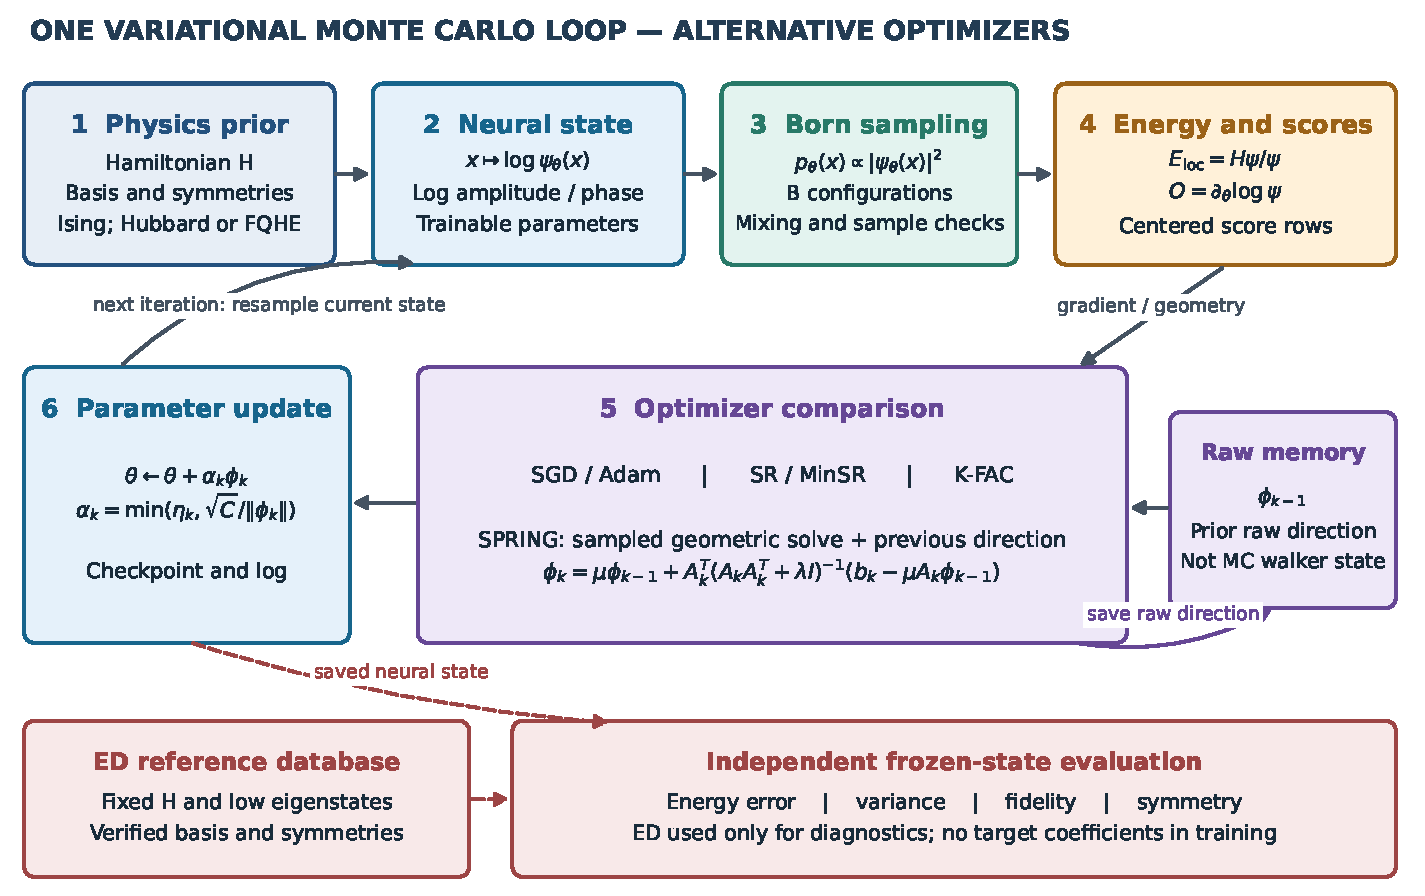
\includegraphics[width=\textwidth]{spring_optimizer_workflow.pdf}
\caption{A shared workflow for strongly correlated quantum systems: begin with Ising, then select Hubbard or FQHE as an advanced problem. Domain knowledge defines the Hamiltonian and wavefunction family; a network learns its parameters from Born-sampled local energies. Optimizers share the physical objective and estimator convention. SPRING direction memory is separate from Markov-chain walker state. ED enters only frozen-state evaluation, without target coefficients in training.}
\end{figure}

\topic{The sampled geometric problem}
For a batch of $B$ configurations and $P$ real parameters, center the complex scores and local energies. Define
\begin{equation}
 A_k=\frac1{\sqrt B}\begin{pmatrix}\operatorname{Re}\delta O\\\operatorname{Im}\delta O\end{pmatrix}
 \in\R^{2B\times P},\qquad
 b_k=-\frac1{\sqrt B}\begin{pmatrix}\operatorname{Re}\delta E_{\rm loc}\\\operatorname{Im}\delta E_{\rm loc}\end{pmatrix},
 \qquad A_k^TA_k=\widehat S,\quad A_k^Tb_k=-\widehat g/2.
\end{equation}
Real states require only $B$ rows. With $\lambda>0$ and raw direction memory $0\leq\mu<1$, the regularized SPRING step is
\begin{align}
 \phi_k&=\mu\phi_{k-1}+A_k^T(A_kA_k^T+\lambda I)^{-1}
 \bigl(b_k-\mu A_k\phi_{k-1}\bigr),\\
 \theta_{k+1}&=\theta_k+\alpha_k\phi_k,\qquad
 \alpha_k=\min\!\left(\eta_k,\frac{\sqrt C}{\|\phi_k\|}\right).
\end{align}
Equivalently, $\phi_k$ minimizes $\|A_k\phi-b_k\|^2+\lambda\|\phi-\mu\phi_{k-1}\|^2$.
The centered null directions are stabilized in the implementation. $\lambda$ is optimizer damping; $\sqrt C$ is the update-norm radius (the package's \texttt{max\_norm}). Store the unscaled direction before the learning-rate/cap operation. The controlled $\mu=0$ case is damped SR/MinSR. A larger batch supplies more sampled rows, but does not replace more parameter updates or guarantee independent samples.

\clearpage
\fancyhead[L]{\small Appendix B: preliminary ED database and NN examples}
\begin{center}{\Large\bfseries B. Preliminary ED benchmarks and NN examples}\end{center}
\textbf{Present database size.} Eleven Hamiltonian instances contain \TotalConfigRows\ configuration rows: \IsingConfigRows\ Ising and \FQHEConfigRows\ FQHE. Counts sum rows per instance; the same 64-row Ising basis is reused at three fields. Tables give decoded input shapes (rows $\times$ columns); FQHE configurations are stored as packed bitstrings. The largest array has $8,512\times22=187,264$ input entries. Ising stores 1,488 eigenvalues across six complete spectra; FQHE stores 98 low eigenpairs across five complete $M=0$ bases. Records include sparse $H$, symmetries, observables and SHA256 provenance. Fidelity is $F=|\langle\psi_0|\psi_\theta\rangle|^2$; ED coefficients serve evaluation only. Hubbard data are proposed.

\begin{center}\small
\begin{minipage}[t]{.48\textwidth}\centering
\textbf{FQHE: pure $V_1$, spherical LLL}\\[3pt]
\begin{tabular}{@{}rrr@{}}\toprule
$N$ & Input shape & $\Delta/V_1$\\\midrule
\FQHEDatabaseRows
\bottomrule\end{tabular}
\end{minipage}\hfill
\begin{minipage}[t]{.49\textwidth}\centering
\textbf{Ising: periodic Pauli, $J=h=1$}\\[3pt]
\begin{tabular}{@{}rrrr@{}}\toprule
$N$ & Input shape & $E_0/J$ & Full gap$/J$\\\midrule
\IsingDatabaseRows
\bottomrule\end{tabular}
\end{minipage}
\end{center}
{\small All listed FQHE ground energies are zero within $1.7\times10^{-16}V_1$, with unique $L=0$ states and uniform density. The $N=8$ neutral gap is $\FQHEGap V_1$ and its first excitation has $L=5$. For Ising $N=6$, the even-sector gap is $2.070552361J$; the database also includes $h/J=0.5,2$. Thirty recorded tests pass (13 FQHE, 17 Ising), including independent pair-projector/sign checks and finite-ring Ising formula checks.}

\begin{figure}[h!]
\centering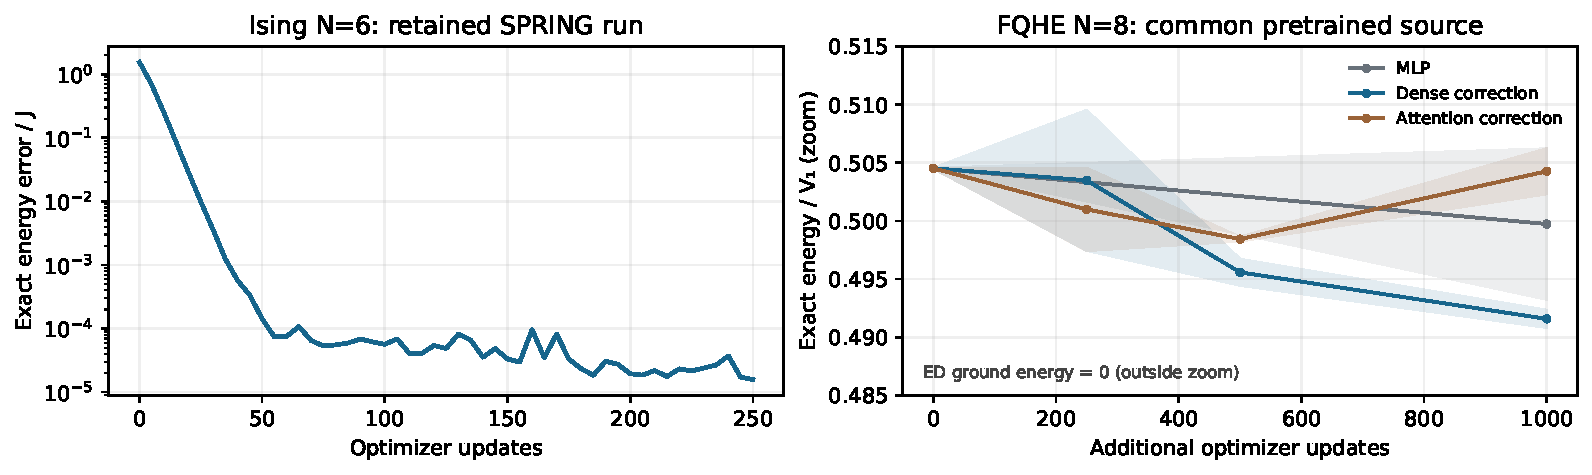
\includegraphics[width=\textwidth]{nn_ed_proposal_examples.pdf}
\caption{Examples from existing SPRING runs, not new optimizer comparisons. Left: exact full-basis Ising energy error during 250 updates ($B=128$). Right: exact FQHE energies during 1,000 additional updates from one common pretrained state ($B=32$); lines show two-seed means and shading their range, not confidence intervals. The FQHE vertical axis is zoomed; the ED ground energy is zero. MLP has only endpoint evaluations, while correction models also have intermediate checkpoints.}
\end{figure}

\begin{center}\small
\begin{tabular}{@{}lrrrr@{}}\toprule
Retained state & Parameters & Exact energy error & Fidelity & Variance\\\midrule
Ising $N=6$, 250 updates & 73 & $1.576\times10^{-5}J$ & $\IsingFidelity$ & $2.054\times10^{-4}J^2$\\
FQHE $N=8$, selected dense & 24,606 & $\FQHEEnergy V_1$ & $\FQHEFidelity$ & $0.465712V_1^2$\\\bottomrule
\end{tabular}
\end{center}
\textbf{Saved NN data.} The Ising diagnostic table is $\IsingLogShape$; FQHE trajectory evaluations are $\FQHELogShape$, and six endpoint records form a $\FQHEEndpointShape$ table. Six FQHE checkpoints also supply length-8,512 complex coefficient vectors. These are aggregate diagnostics and predictions, rather than retained raw Monte Carlo batches; the six continuations share one pretrained source.

\textbf{Interpretation.} Ising gives an accurate entry-level example; FQHE illustrates harder convergence. These preliminary runs motivate the staged project. Hubbard needs its own ED and NN runs. Existing timings have different boundaries and do not establish cross-system speedups.

{\footnotesize\raggedright\textbf{Local data:} \path{Final_proj/SPRING_Haldane_FQHE/results/ed_benchmarks/};
\path{Final_proj/SPRING_Ising_test/benchmarks/ed/};
\path{Final_proj/benchmarks/}.\par
Figure inputs and their hashes are recorded in \texttt{proposal\_verified\_data.json}; the accompanying Python script regenerates both figures and numerical table rows.\par}
\fi
\end{document}
